% !TEX root = ../thesis.tex
\chapter{Research}
\label{chapter:<research_number_of_items>}

\section{Introduction}
\label{sec:research_introduction}

The visualization has been proven to be an essential part in the recommendation since it can determine if it is useful or not from the user point of view \cite{trust-building}. There have been studies to determine how an item should be presented to the user in order to gain his/her attention as described in section \ref{sec:Presentation} but there are not been much documented studies about the number of items that a recommendation system should display in order to maximize the user perception of a good recommendation.

Thus the proposal of this research is to evaluate how the number of movie visualized alter the user perception of a good or bad recommendation. To be scientific valid only one variable of the system should vary between all the test groups. In this case the number of items displayed has been chosen to vary between 2, 5 and 10 with at least 30 samples (or completed surveys) each. This is also the first research done using the Movish automatic recommendation survey system.  

As for algorithm pureSVD has been chosen because it has been proved to have the best performances between all the algorithms supported by the Movish system \cite{performance-recommender-algorithms}. PureSVD was the top performer in both Movielens and Netflix \cite{netflixprize} datasets beating more detailed and sophisticated latent factor models even if it is one of the simplest algorithms available.

In section \ref{sec:research_sources} the reader will be guided in analyzing the various sources used, in section \ref{sec:research_survey} a complete survey for this research is exposed. Then in section \ref{sec:research_analysis} the analysis of the data is published and section \ref{sec:research_conclusions} exposes the conclusions.

\section{Sources}
\label{sec:research_sources}

For this research a number of different resources has been used in order to collect the maximum number of surveys with the minimum budget. Aside of Amazon Mechanical Turk of which we discussed on secion \ref{sec:crowdsourcing}, also Facebook and Google plus have been used in order to test if a survey can go viral on social networks.

In order to maximize the user attention a whiteboard rewarding an eligibility of prize to the ones that perform the survey has been used. The Facebook post that promoted one of the three surveys that have been performed is displayed in figure \ref{fig:facebook_survey}.

\begin{figure}
  \centering
  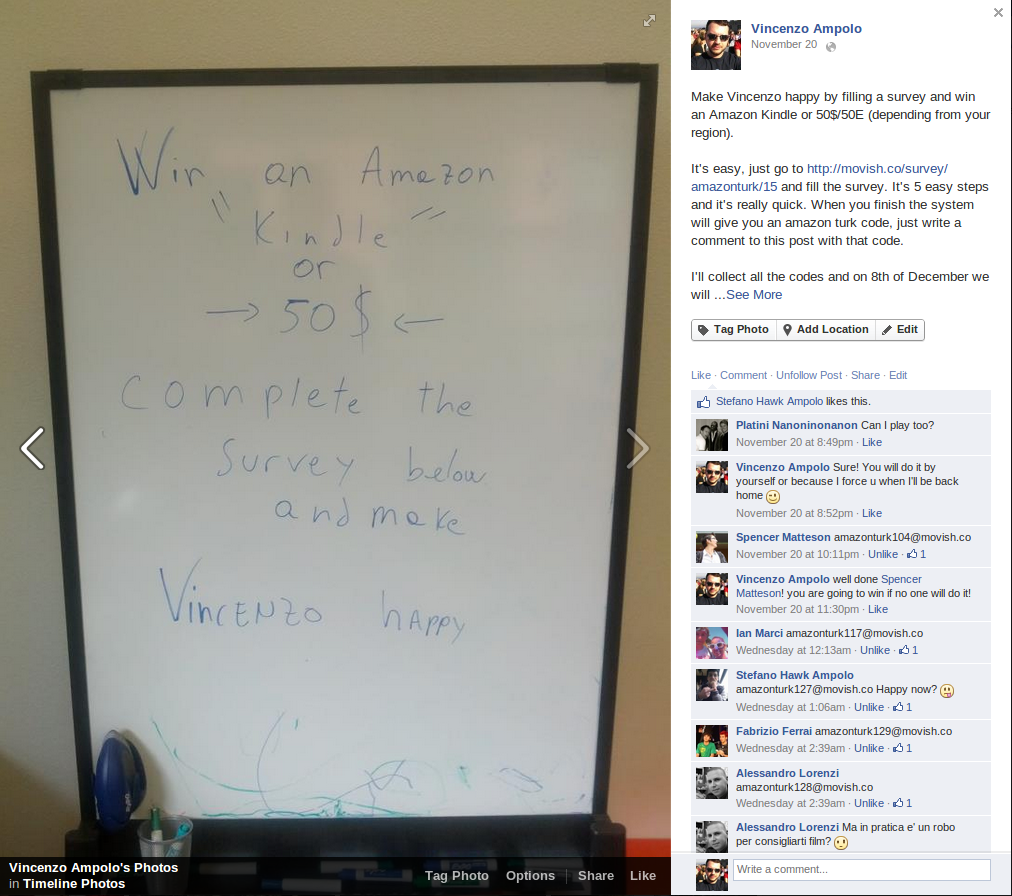
\includegraphics[width=\textwidth]{figures/facebook_survey.png}
  \caption{Facebook post to participate to a survey}
  \label{fig:facebook_survey}
\end{figure}

The whiteboard message is: \textit{Win an Amazon Kindle or \$50, complete the survey below and make Vincenzo happy}. The message had two goals: stimulate all my close friends in taking action in order to help me in my research and to stimulate all the not close friends in performing the survey due to the prize they could win. In order to be eligible for the prize the user/friend had to write the Amazon Mechanical Turk code that is displayed at the end of the survey as comment to the post.  The same message has been posted on Google plus and can be seen in figure \ref{fig:google_plus_survey}.

\begin{figure}
  \centering
  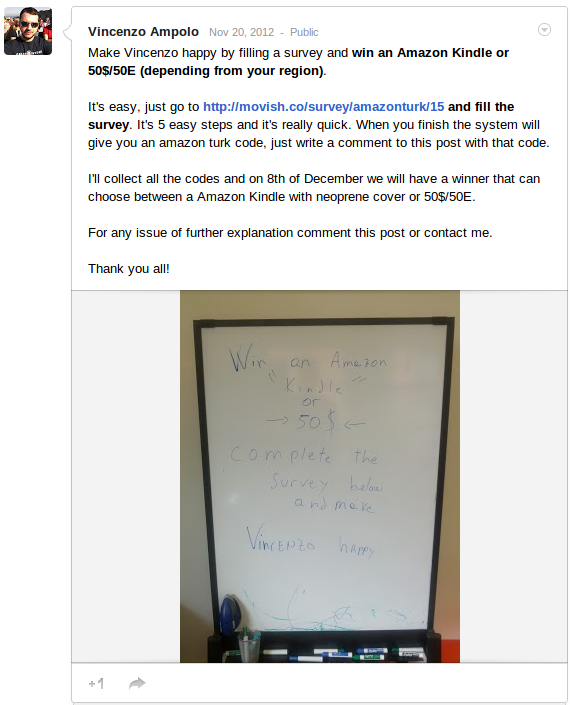
\includegraphics[width=\textwidth]{figures/google_plus_survey.png}
  \caption{Google plus post to participate to a survey}
  \label{fig:google_plus_survey}
\end{figure}

The facebook post was able to retrieve a total 13 users performing the survey of which 7 of them can be categorized as not close friends. The Google plus post wasn't able to stimulate any user.

\section{Survey}
\label{sec:research_survey}

In order to fulfill the goal of this research a survey type of \textbf{algorithm\_strength} with 5 free ratings using \textbf{pureSVD} algorithm has been chosen. The reason of this choice are explained in section \ref{sec:research_introduction}. The survey starts asking general demographic information as shown in figure \ref{fig:survey_phase_1}.

\begin{figure}
  \centering
  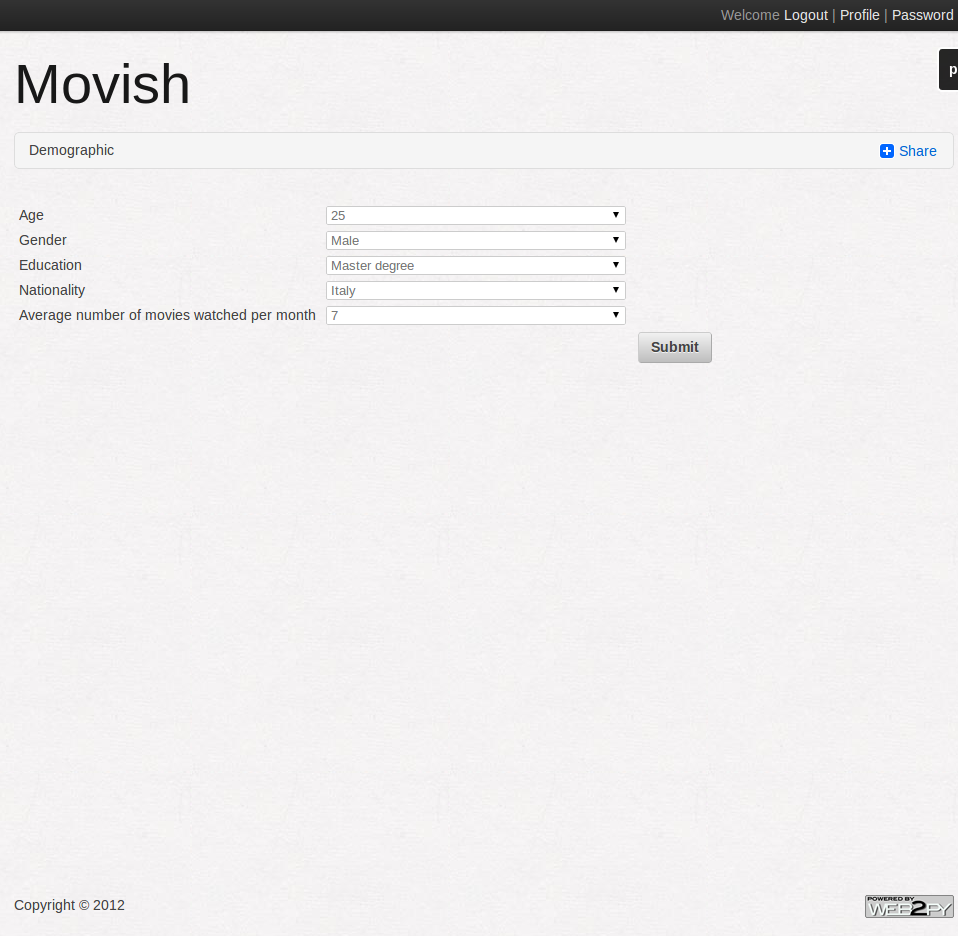
\includegraphics[width=\textwidth]{figures/survey_demographic.png}
  \caption{Survey phase 1}
  \label{fig:survey_phase_1}
\end{figure}

The user is asked to put the age, the gender, the education type, the nationality and the average numbers of movies watched per month. The goal of those questions is to associate the user with a cluster of users since the preference for a special category of movies change in respect of the age and the nationality. The average number of movies watched per month is an indicator to test if the user likes, in general, watching movies.

\begin{figure}
  \centering
  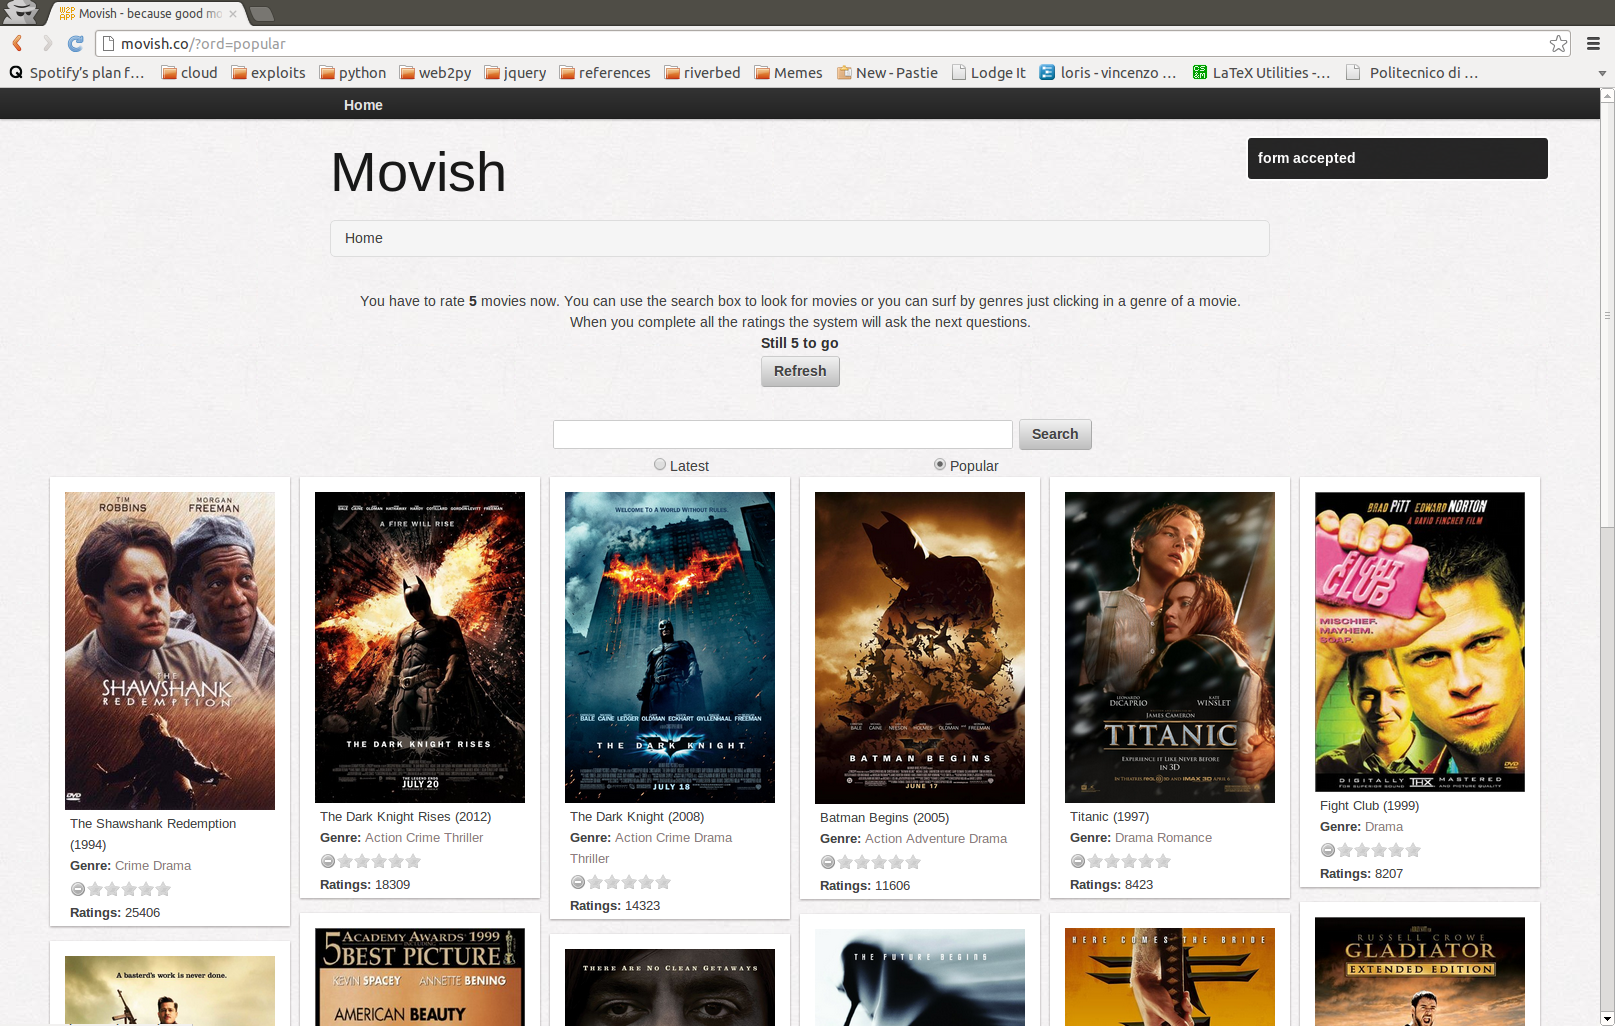
\includegraphics[width=\textwidth]{figures/free_ratings.png}
  \caption{Survey phase 2}
  \label{fig:survey_phase_2}
\end{figure}

After the demographic questions the user is able to perform the free ratings from the page shown in figure \ref{fig:survey_phase_2}. From this page the logout link in the top right part of the page disappear: the user which is performing the survey is not supposed to logout anymore. Beside this also all the not useful links that may lead the user out of the Movish system are removed in order to force the user in completing the survey before leaving the system.

To facilitate the user in starting rating movies, the top 15 movies with ratings in the system are chosen and displayed: they represent the top popular movies in the system. The user can rate directly in the homepage thanks to the star system under each movie poster or by going to the movie detail page and rate again from there using the same star system. Optionally the user can also see the trailer and read the plot of a movie in the movie detail page shown in figure \ref{fig:movie_detail}.

User is also allowed to use the search box to look for any movie he/she wants. In fact this way of looking to the items is suggested by the top message of the page. It is so to test the completeness of the catalog. After the user rated the number of free ratings chosen by the administrator at survey creation discussed in section \ref{sec:survey_creation}, the system automatically redirect the user to the next page of the survey, the catalogue questions.

\begin{figure}
  \centering
  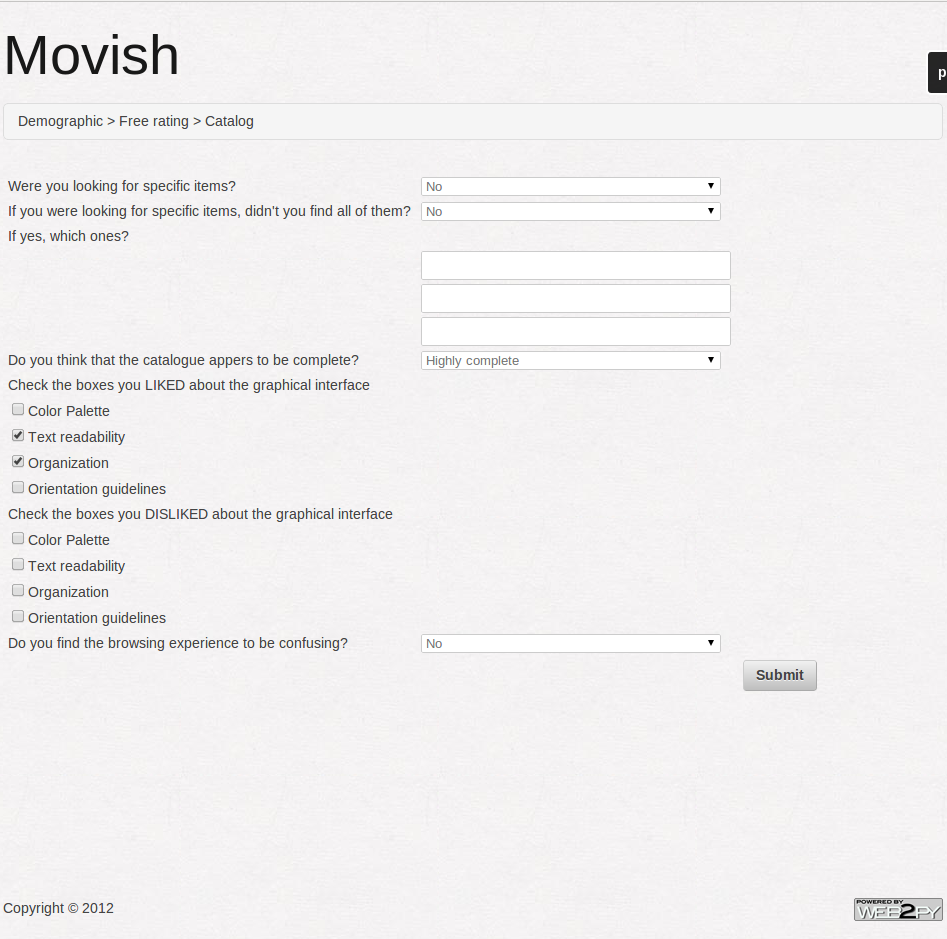
\includegraphics[width=\textwidth]{figures/survey_catalog.png}
  \caption{Survey phase 3}
  \label{fig:survey_phase_3}
\end{figure}

These questions are shown in figure \ref{fig:survey_phase_3}. The user is asked to answer some questions related to the catalogue he/she just browsed doing the free ratings. He/she has to answer questions about the browsing experience: looking for specific movies or not, if some movies were not found, to list their names, the completeness of the catalogue and what he/she liked about the website about color palette, text readability, organization and orientation guidelines. After submitting the form the user is redirected to the next phase, the recommendation. 

\begin{figure}
  \centering
  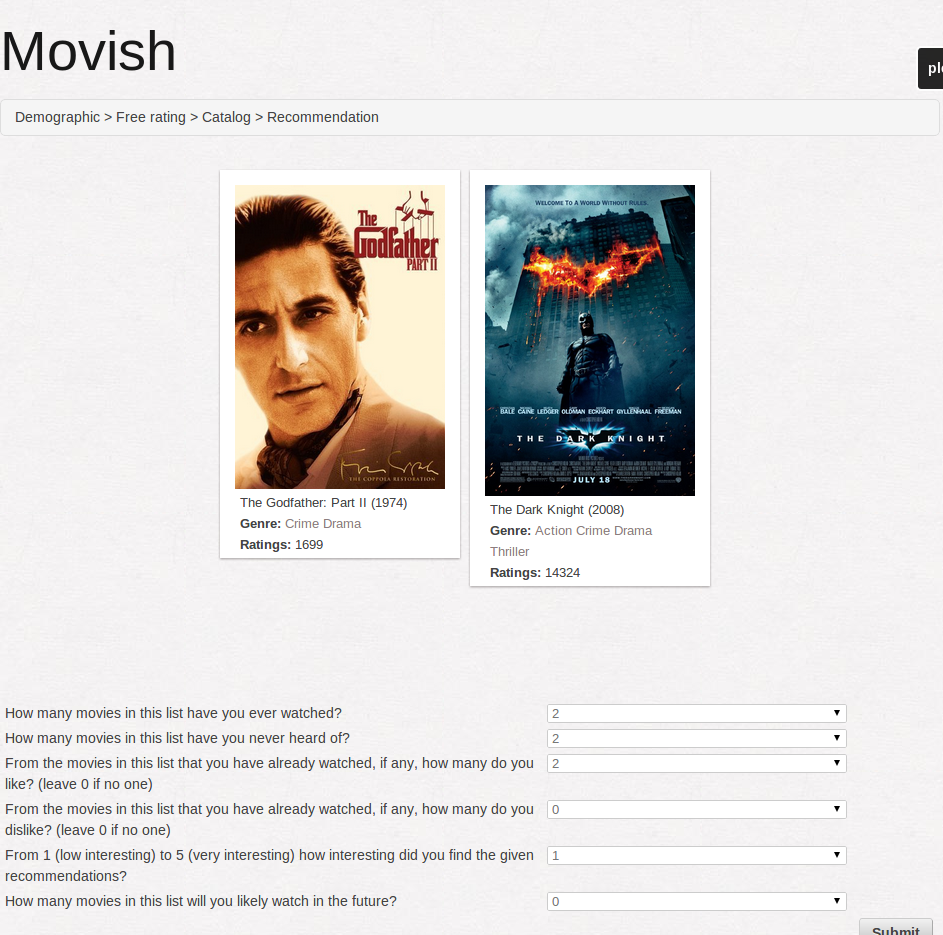
\includegraphics[width=\textwidth]{figures/survey_recommendation.png}
  \caption{Survey phase 4}
  \label{fig:survey_phase_4}
\end{figure}

It is shown in figure \ref{fig:survey_phase_4}. In order to have a better image for this thesis, the survey with only two recommendation has been chosen. The number of movies displayed in this phase are 2,5 or 10 depending from which specific survey the user is performing. All the not necessary links are removed. The user cannot see the details of a movie either or click on the genres of a movie to perform a search. Given the poster and the title of the movies in the list only the user has to ask question regarding the number of movies watched, the number of movie the user have heard of, the number of watched movies the user likes or dislikes, the recommendation sentiment or if the recommendation is useful for the user or not, which is the main question leading this research and the number of movies from the recommendation that the user will be likely to watch.  

\begin{figure}
  \centering
  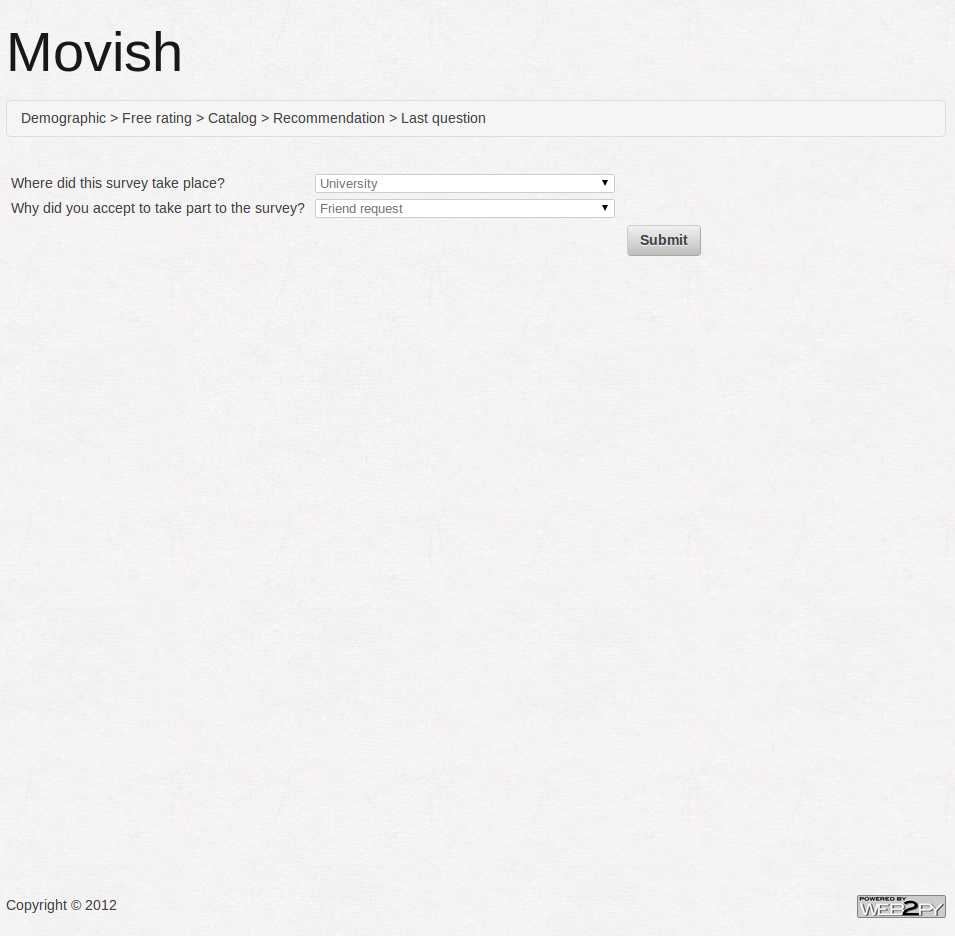
\includegraphics[width=\textwidth]{figures/survey_localinfo.png}
  \caption{Survey phase 5}
  \label{fig:survey_phase_5}
\end{figure}

After submitting the recommendation form the user is redirected to the last questions shown in figure \ref{fig:survey_phase_5}. The user is asked of inserting the place in which the survey is taking place and why the user is performing the survey.

\section{Analysis}
\label{sec:research_analysis}

The data of the survey can be retrieved from the survey list of the admin interface described in section \ref{sec:admin_interface} by clicking oon the ``download results'' icon after the \textit{Amazon Turk link} column.

For this kind of research the feeling of a good recommendation, such as the rating of the recommendation list, is the driver value of the research. So the first way to look at the data is to count the number of equal ratings and plot them in a barchart, one for each survey. This data is available from the questions of the survey at the question regarding the usefulness of the recommendation.

\begin{figure}
  \centering
  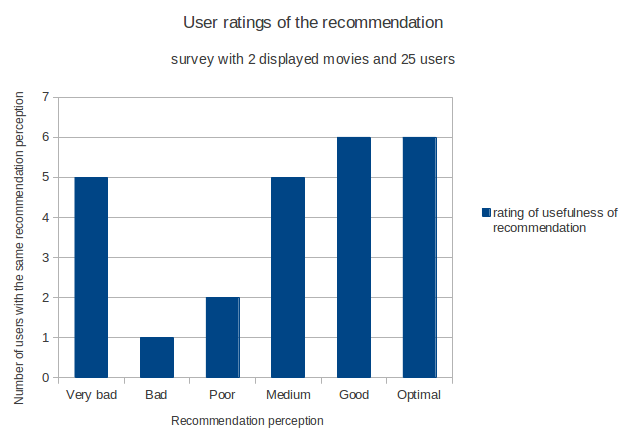
\includegraphics[width=\textwidth]{figures/survey2_graph1.png}
  \caption{Survey having two displayed movies}
  \label{fig:survey2}
\end{figure}

Figure \ref{fig:survey2} shows the number of users grouped by the rate on the recommendation or the usefulness of the recommendation. The first results that highlights in that graph is the fact that over 25 surveys, displaying 2 movies resulted in a very bad recommendation for 5 users. It was also very good for 12 users (summing the \textit{good} and \textit{optimal} columns). The \textbf{average} of all the ratings is \textbf{2.96}, the \textbf{standard deviation} is \textbf{1.84}.   

\begin{figure}
  \centering
  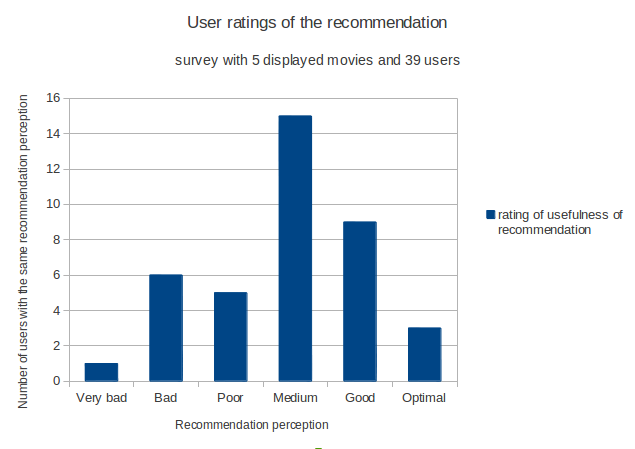
\includegraphics[width=\textwidth]{figures/survey5_graph1.png}
  \caption{Survey having five displayed movies}
  \label{fig:survey5}
\end{figure}

Figure \ref{fig:survey5} shows the same graph for the second survey, the one displaying 5 movies at time while the user has to answer the question about the usefulness of the recommendation. A big amount of users thinks that the recommendation has medium usefulness. The big difference with the previous data is that the number of very bad recommendation is down to only one case and that the number of users that declare that the recommendation is optimal (score of 5) is significantly dropped. The \textbf{average} of all the ratings is \textbf{2.87} and the \textbf{standard deviation} is \textbf{1.24}.

\begin{figure}
  \centering
  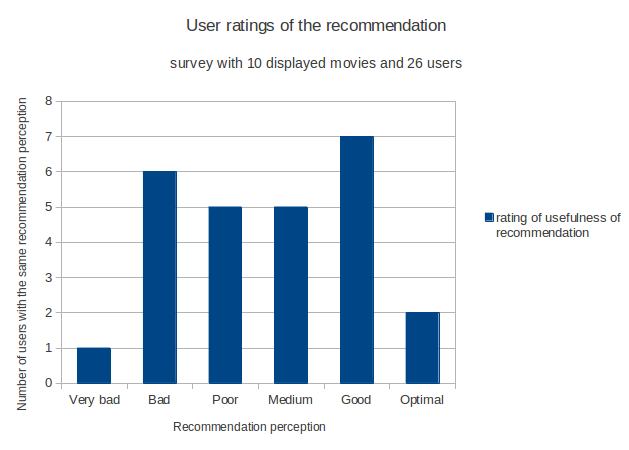
\includegraphics[width=\textwidth]{figures/survey10_graph1.png}
  \caption{Survey having ten displayed movies}
  \label{fig:survey10}
\end{figure}

Figure \ref{fig:survey10} shows the same graph for the third survey instead, the one in which the user sees 10 movies at the time the user has to rate the recommendation he/she received. In this graph the number of user that rate the recommendation very bad is low like in the survey with 5 movies displayed but the number of people that rated the recommendation as poor is the same as the people that rated the recommendation to be medium. The \textbf{average} of all the ratings is \textbf{2.65} and the \textbf{standard deviation} is \textbf{1.41}.

Due to the nature of the surveys and the different scale (each survey has a different number of samples or people that performed the survey), to better analyze this data considering the average as the primary driver and a higher standard deviation as a noise factor. Using the signal to noise ratio defined as 
\begin{math}
SNR=\mu/\sigma  
\end{math}
every survey can be reduced to a single scalar indicating which survey that had a different number of displayed movie was the best for the users. This leads to data in figure \ref{fig:research_signal_to_noise}

\begin{figure}
  \centering
  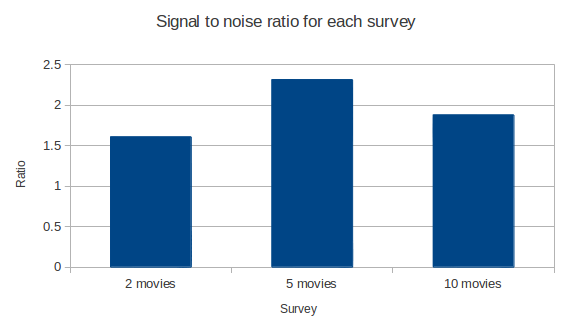
\includegraphics[width=\textwidth]{figures/research_signal_to_noise_ratio.png}
  \caption{Signal to noise ratio for the three surveys}
  \label{fig:research_signal_to_noise}
\end{figure}

These are the
\begin{math}
  SNR
\end{math}
for each survey:
\begin{itemize}
\item \textit{Survey with two displayed movies}: \begin{math}1.61\end{math}
\item \textit{Survey with five displayed movies}: \begin{math}2.31\end{math}
\item \textit{Survey with ten displayed movies}: \begin{math}1.88\end{math}
\end{itemize}

This last graph shows how each survey performs in terms of user likeliness of the recommendation based on the number movies displayed during the recommendation phase. The higher is the bar, the better is the survey.

\section{Conclusions}
\label{sec:research_conclusions}

This research wanted to prove if the usefulness of a recommendation depends on the number of items that are displayed to the user. In order to perform the research three surveys with the same recommendation algorithm have been submitted to 90 different users using Amazon Mechanical Turk and Facebook. The only difference between the surveys was the different number of movies displayed during the recommendation. The first survey had two displayed movies, the second one had five movies and the third one had ten movies. 
The collected data showed a relation between the different number of movie displayed and the usefulness of the recommendation itself. After further study, considerations and calculating the mean and the standard deviation the three surveys have been compared using the signal to noise ratio.
This lead the survey with five movies displayed to be the one that the user prefer compared to the one with two or ten. If there wouldn't be any relation between the number of displayed movies and usefulness of the recommendation there wouldn't be any significant difference in the average usefulness of the recommendation and its standard deviation. 

\acresetall